%!xelatex = 'xelatex --halt-on-error %O %S'

\documentclass{thuemp}
\usepackage{url}
\usepackage{lipsum}  % 生产假书乱文的包,实际使用时可去掉
\usepackage{hyperref}
\begin{document}

% 标题,作者
\emptitle{PID 控制在医学麻醉过程血压控制中的应用}
\empauthor{秦华谦}{李中华老师}

% 奇数页页眉 % 请在这里写出第一作者以及论文题目
\fancyhead[CO]{{\footnotesize 秦华谦: PID 控制在医学麻醉过程血压控制中的应用}}


%%%%%%%%%%%%%%%%%%%%%%%%%%%%%%%%%%%%%%%%%%%%%%%%%%%%%%%%%%%%%%%%
% 关键词 摘要 首页脚注
%%%%%%%%关键词
\Keyword{PID控制, 麻醉, 血压控制}
\twocolumn[
\begin{@twocolumnfalse}
\maketitle

%%%%%%%%摘要
\begin{empAbstract}
本文基于PID控制系统开发了一个系统,旨在自动测量和控制多种生命参数,以保持其在适当范围内。其目标是提高手术中麻醉师的安全性。为了进一步优化系统性能,我们进行了一项专门的研究,通过对kp、ki、kd三个参数的调整,探究PID系统内不同参数对系统响应的影响。该系统实现了自动调节麻醉深度,以减小波动和冲击响应。实验结果表明,引入设计的控制器后,血压控制系统对于给定输入信号的超调量减小,调节时间缩短。在阶跃输入信号下的稳态误差为零,并在阶跃扰动输入信号下能保持稳态误差在一定范围内,最终实现稳态输出为零。
\end{empAbstract}

%%%%%%%%英文标题、作者、摘要、关键词
\emptitleEn{Application of PID control in blood pressure control in medical anesthesia process}
\empauthorEn{Huaqian Chin}{Prof. Li Zhonghua}
\KeywordEn{PID control, Anaesthetization, Blood Pressure Pontrol}

\begin{empAbstractEn}
This article has developed a system based on the PID control system, aimed at automatically measuring and controlling various vital parameters to maintain them within an appropriate range. The goal is to enhance the safety of anesthesiologists during surgery. To further optimize system performance, we conducted a dedicated study, investigating the impact of different parameters in the PID system on system response by adjusting the kp, ki, and kd parameters. The system achieves automatic adjustment of anesthetic depth to minimize fluctuations and impact responses. Experimental results show that after introducing the designed controller, the overshoot of the blood pressure control system for a given input signal decreases, and the adjustment time shortens. The steady-state error under step input signals is zero, and under step disturbance input signals, it can maintain the steady-state error within a certain range, ultimately achieving a steady-state output of zero.
\end{empAbstractEn}

%%%%%%%%首页角注,依次为实验时间、报告时间、学号、email
\empfirstfoot{2023-05-20}{2023-5-30}{21312683}{qinhq5@mail2.sysu.edu.cn}
\end{@twocolumnfalse}
]
%%%%%%%%!首页角注可能与正文重叠,请通过调整正文中第一页的\enlargethispage{-3.3cm}位置手动校准正文底部位置:
%%%%%%%%%%%%%%%%%%%%%%%%%%%%%%%%%%%%%%%%%%%%%%%%%%%%%%%%%%%%%%%%
%  正文由此开始
\wuhao 
%  分栏开始

\section{引~~言}
\enlargethispage{-3.3cm}
手术中麻醉师需监测多种生命参数,如:麻醉
深度、血压、心率、体温、血氧、呼气中二氧化碳
浓度等,并将它们控制在适当的范围内。能够自动
测量、控制某些生命参数,能够提高受术者的安
全。我们希望开发一个自动调节麻醉深度的系
统,病人的安全是最终目标。

许多麻醉师将平均动脉压作为麻醉深度最可
靠的度量。根据临床经验和麻醉师所遵从的程序,
被控变量确定为平均动脉压(MAP)。

本文主要是运用 PID 控制器的设计方法,对
麻醉过程中的血压控制模型进行控制器的设计,通过对kp、ki、kd三个参数的调整,探究PID系统内不同参数对系统响应的影响。
并且针对 PI,PD,PID 三种控制器在有无扰动两种情况下
进行性能分析的比较。

\section{实验原理}


\subsection{PID控制原理}

PID控制是一种常用的反馈控制算法,用于调节和稳定系统的输出。它的名称代表比例(Proportional)、积分(Integral)和微分(Derivative),分别表示控制器的三个主要组成部分。

比例控制(Proportional Control)是PID控制的基本部分之一。它通过将当前误差与一个比例常数相乘,产生一个控制量,用于调节系统输出。比例控制的作用是使系统对误差做出直接的响应,但它无法解决误差积累和系统超调等问题。

积分控制(Integral Control)是PID控制的第二个组成部分。它将误差的积分值与一个积分常数相乘,产生一个控制量。积分控制的作用是消除稳态误差,即系统输出与期望输出之间的差异。通过积分控制,系统可以逐渐减小并消除持续的误差。

微分控制(Derivative Control)是PID控制的最后一个组成部分。它通过将误差的变化率与一个微分常数相乘,产生一个控制量。微分控制的作用是抑制系统的超调和振荡,并提高系统的响应速度。通过微分控制,系统可以更快地调整输出,以适应误差变化的速率。

PID控制器将比例、积分和微分控制相结合,通过对误差的不同方面进行调节,实现对系统输出的精确控制。PID控制器的输出值由三个控制分量的加权和得出,即:

输出 = 比例控制 + 积分控制 + 微分控制

通过调整比例常数、积分常数和微分常数,可以对PID控制器进行参数调优,以满足不同系统的需求。调优过程通常包括实验、观察和调整,以获得最佳的控制效果。

总而言之,PID控制是一种基于反馈的控制算法,通过比例、积分和微分控制三个部分的相互作用,实现对系统输出的精确调节。它广泛应用于自动控制领域,用于稳定系统、消除误差和提高响应速度。

\subsection{系统设计流程图}
\begin{figure}[H]
\centering
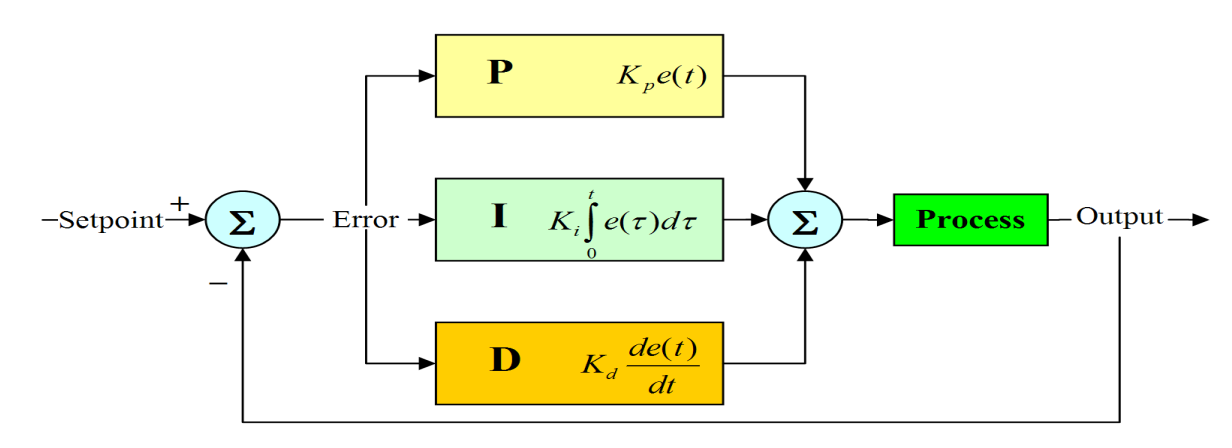
\includegraphics[width=1\linewidth]{./img/from_internet/PID.png}
\end{figure}

\subsection{系统参数介绍}

PID 控制器的比例单元 (P)、积分单元 (I) 和微分单元 (D) 分别对应目前误差、过去累计误差及未来误差。借由调整 PID 控制器的三个参数,可以调整控制系统,设法满足设
计需求。

PID控制器(比例-积分-微分控制器)的参数选择取决于具体的应用场景和系统的动态特性。通常,这些参数需要通过一些调参方法(例如Ziegler-Nichols方法)进行调整,以达到系统的稳定性和性能需求。

PID控制器的三个参数分别为:

1. P(比例):该参数控制系统的响应速度。P参数越大,系统对错误的反应越快,但如果过大,可能会导致系统不稳定。

2. I(积分):该参数控制系统是否能达到设定点(或称为参考点)。I参数可以消除系统的静差,但如果过大,可能会导致系统超调和震荡。

3. D(微分):该参数控制系统的稳定性。D参数可以预测系统的行为,减小系统的超调,但如果过大,可能会引入噪声,使系统不稳定。

在实际应用中,PID参数的调整是一项复杂的工程任务,需要根据系统的具体特性和性能需求进行优化。有时,人们也使用一些自适应的PID控制算法,如模糊PID,遗传算法等,以自动地优化PID参数。


\section{实验过程}

\subsection{系统设计流程图}
\begin{figure}[H]
\centering
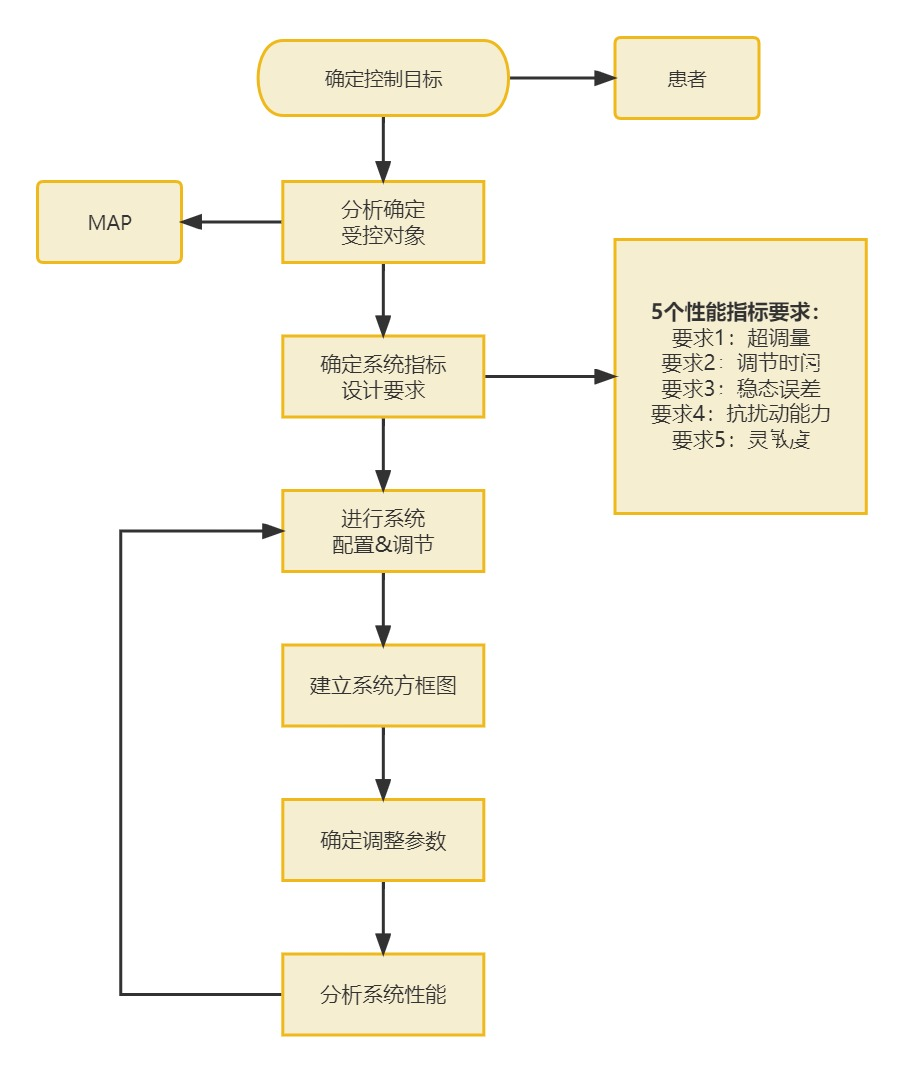
\includegraphics[width=1\linewidth]{./img/work_stream.jpg}
\end{figure}

\subsection{控制目标与实验要求}

\subsubsection{麻醉过程中的血压控制系统控制目标}
\begin{itemize}
	\item 控制对象: 需麻醉的患者
	\item 控制任务: 将患者 MAP 调节到任意预期设定的水平,并在存在干扰信号的情况下将 MAP维持在预期设定的水平。
	\item 受控变量: MAP(平均动脉压)
	\item 系统输入:MAP的期望值
	\item 干扰输入: 手术干扰,噪声干扰
	\item 误差量: 稳态误差 = 输入 - 输出
	\item 系统输出: 实际的 MAP 量
\end{itemize}

\subsubsection{该控制系统的实验设计要求}
\begin{enumerate}
	\item 取N(s)=0, Td(s)=0
	
  \begin{itemize}
    \item 基于PD、 PI控制器对系统进行Matlab仿真。
    
    \begin{itemize}
      \item 在PD或PI控制器中,固定一个参数,调节另外一个参数,观察输出结果的变化
    \end{itemize}

    \item 基于PID控制器对系统进行Matlab仿真
    \begin{itemize}
      \item 改变三个参数的值,看在不同的组合下,观察系统的输出的变化
    \end{itemize}
    
  \end{itemize}

	\item 取N(s)=0, Td(s)=50/s
	\begin{itemize}
    \item 重复上面的仿真过程
  \end{itemize}
  
\end{enumerate}



\subsection{系统设计}

其中, $R(s)$和$Y (s)$分别为期望的平均动脉压变化和实际的平均动脉压变化, 
两者的偏差被控制器用于确定对泵的阀门给定值,泵/蒸发器给患者输送麻醉蒸汽。
而$𝑇𝑑(s)$和$𝑁(s)$分别为手术过程中的扰动和噪声, $G_c (s)$为待加入的控制器传递函数。
另外, G(s)是被控对象, 其传递函数为
\begin{equation}
G(s)=1/(s+p)^2\
\end{equation}

传感器H(s)传递函数为
$$ H\left(s\right)=1 $$

泵的传递函数为$G_p(s)$,为
$$ G_{p\left(s\right)}=\frac{U(s)}{V(s)}=\frac{1}{s} $$

\subsection{传递函数设计与解析}

通过对信号方框图的分析,我将$R \& Td \& N$分别作为输入,重绘信号方框图

\begin{figure}[H]
\centering
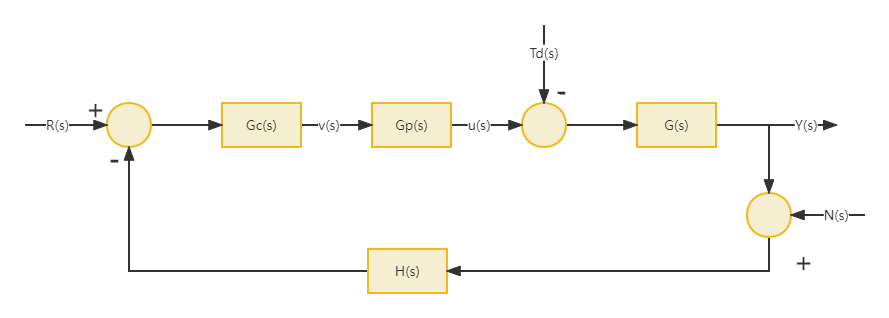
\includegraphics[width=1\linewidth]{./img/Rs.png}
\caption{$Rs(s)$作为输入} 
\end{figure}

\begin{figure}[H]
\centering
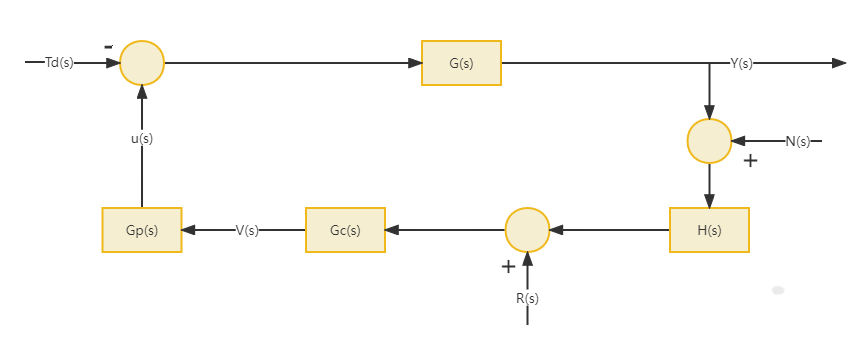
\includegraphics[width=1\linewidth]{./img/Td.png}
\caption{$Td(s)$作为输入} 
\end{figure}

\begin{figure}[H]
\centering
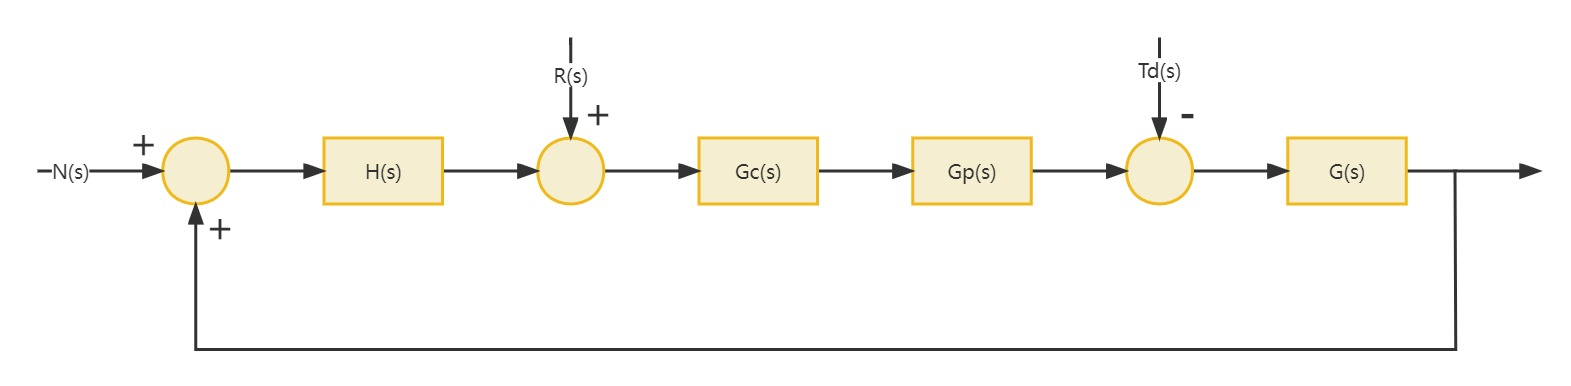
\includegraphics[width=1\linewidth]{./img/N.jpg}
\caption{$N(s)$作为输入} 
\end{figure}

根据三幅信号框图,写出闭环传递函数如下:

以$R(s)$作为输入
$$
\emptyset_r(s)=\frac{G_c(s)\ast G_p(s)\ast G(s)}{1+H(s)\ast G_c(s)\ast G_p(s)\ast G(s)}
$$
以$R(s)$作为输入
$$
\emptyset_{Td}\left(s\right)=\frac{G(s)}{1+H\left(s\right)\ast G_c\left(s\right)\ast G_p\left(s\right)\ast G\left(s\right)}
$$
以$R(s)$作为输入
$$
\emptyset_n(s)=\frac{H(s)\ast G_c(s)\ast G_p(s)\ast G(s)}{1+H(s)\ast G_c(s)\ast G_p(s)\ast G(s)}
$$

\subsection{PID系统传递函数}
$$
G_c\left(s\right)=\frac{K_ds^2+K_ps+K_i}{s}
$$

\subsection{仿真细节与结果展示}
% ==================================================================
\subsubsection{原系统}
取N(s)=0, Td(s)=0, R(s)=10/s

可以看到先对未加入 pid 控制器的系统进行响应分析,通过 matlab 运行程序,作图,得到原系统的阶跃输入

当到达绿线时,系统给予了一个$R(s)=10/s$的阶跃输入,可以看到几乎没有超调量,到达红线时
输出进入5\%的误差带,调节时间$t_s = 12$
\begin{figure}[H]
\centering
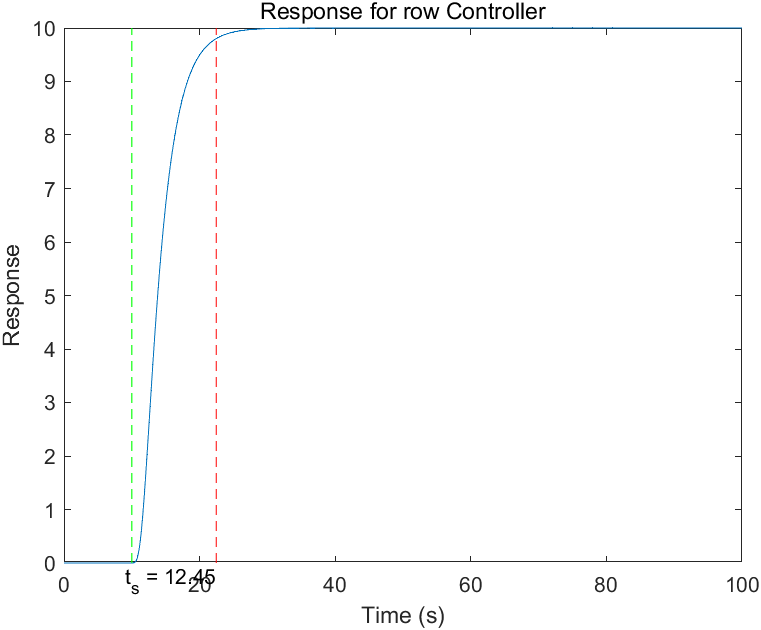
\includegraphics[width=1\linewidth]{./img/None_p1_R.png}
\end{figure}

取N(s)=0, Td(s)=50/s, R(s)=10/s

测试系统在阶跃扰动的情况下的性能,在t=0的时候给予一个R(s) = 10/s的输入,
在t=50的时候给予一个Td(s) = 50/s的阶跃扰动,观察超调量,作图如下

超调量过大

\begin{figure}[H]
\centering
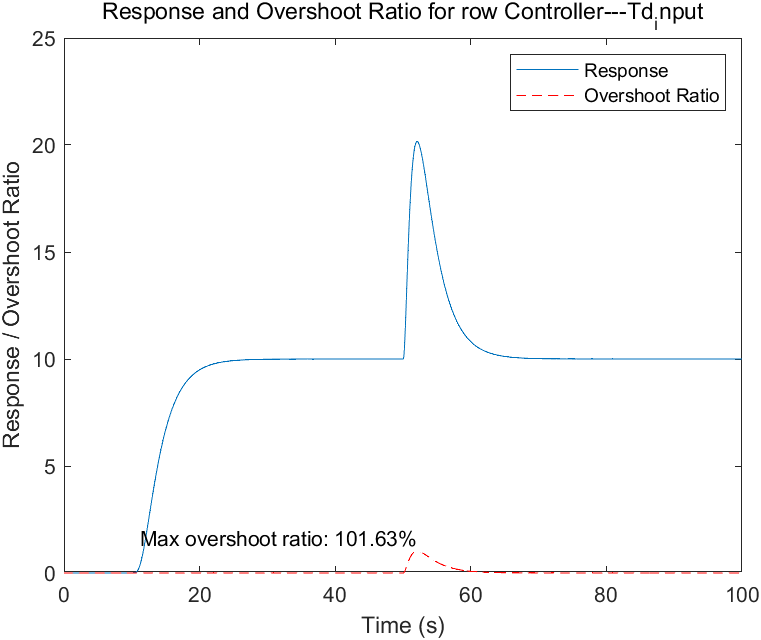
\includegraphics[width=1\linewidth]{./img/None_p2_Td.png}
\end{figure}

% ==========================================================================================
\subsubsection{PI控制器}
参数:R = 10 (t>10);  N(s) = 0;  Td(s) = 0;

在这个模块中,将PI控制器接入了系统的Gc(s)的位置

实现了对两个参数 (Kp \& Ki) 进行了两组分析
\begin{enumerate}
  \item 保持Ki不变,调整Kp的值————以0.8为步长,在[0.8,4]的范围内生成5张系统时域图
  \begin{figure}[H]
    \centering
    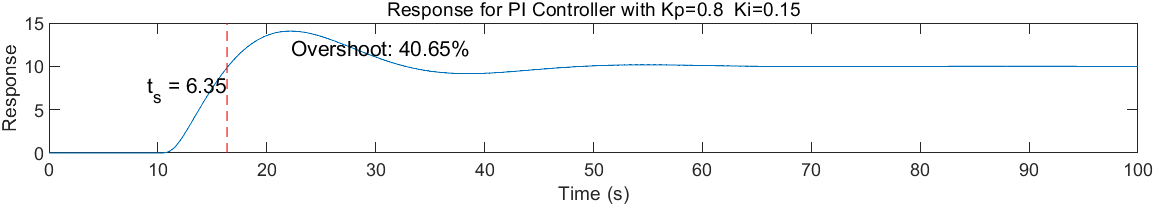
\includegraphics[width=1\linewidth]{./img/PI/i1.png}
  \end{figure}
  \begin{figure}[H]
    \centering
    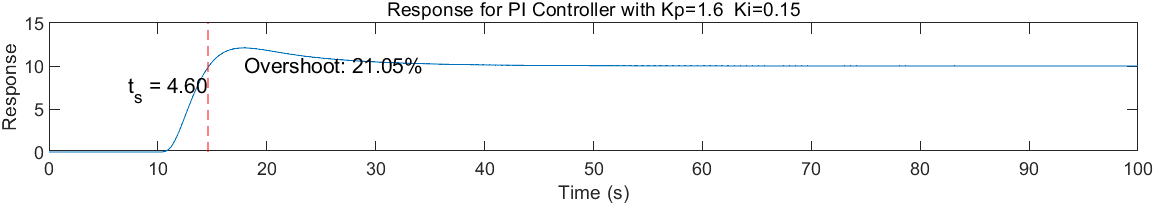
\includegraphics[width=1\linewidth]{./img/PI/i2.png}
  \end{figure}
  \begin{figure}[H]
    \centering
    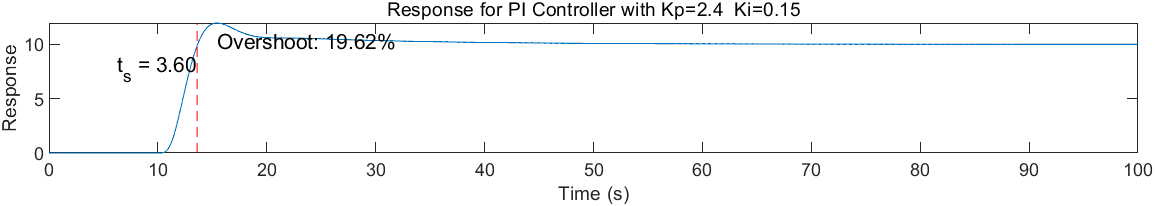
\includegraphics[width=1\linewidth]{./img/PI/i3.png}
  \end{figure}
  \begin{figure}[H]
    \centering
    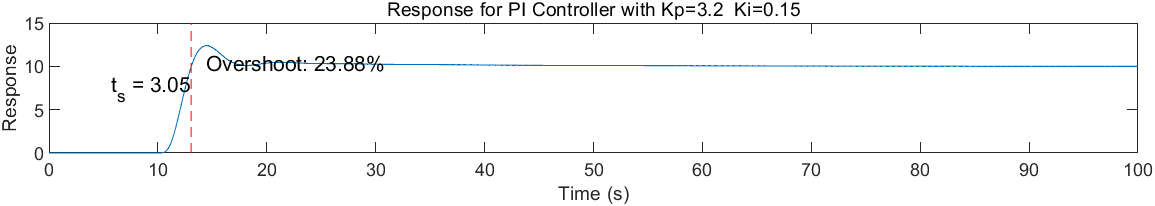
\includegraphics[width=1\linewidth]{./img/PI/i4.png}
  \end{figure}
  \begin{figure}[H]
    \centering
    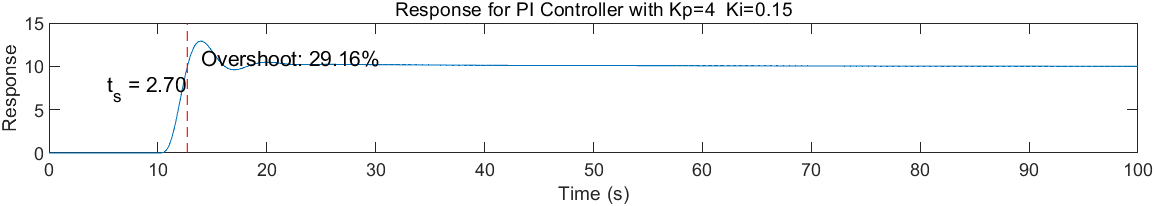
\includegraphics[width=1\linewidth]{./img/PI/i5.png}
  \end{figure}

  \item 保持Kp不变,调整Ki的值————以0.15为步长,在[0.15,0.75]的范围内生成5张系统时域图
  \begin{figure}[H]
    \centering
    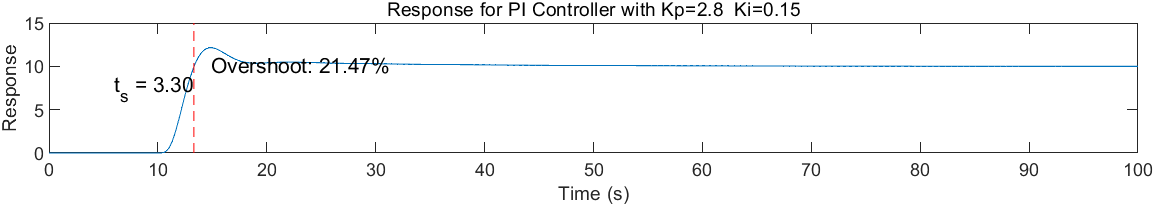
\includegraphics[width=1\linewidth]{./img/PI/p1.png}
  \end{figure}
  \begin{figure}[H]
    \centering
    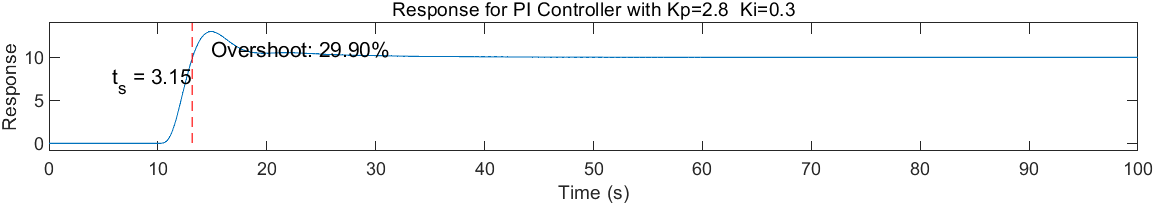
\includegraphics[width=1\linewidth]{./img/PI/p2.png}
  \end{figure}
  \begin{figure}[H]
    \centering
    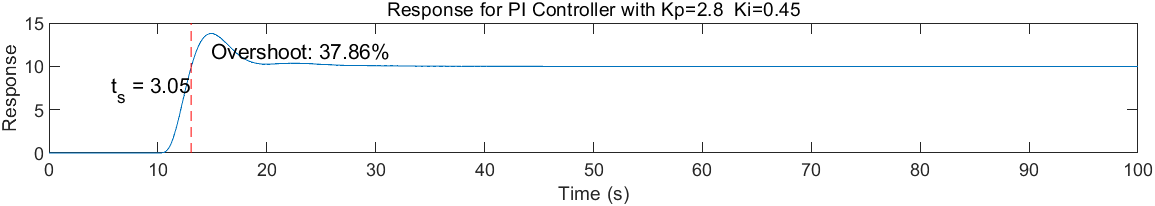
\includegraphics[width=1\linewidth]{./img/PI/p3.png}
  \end{figure}
  \begin{figure}[H]
    \centering
    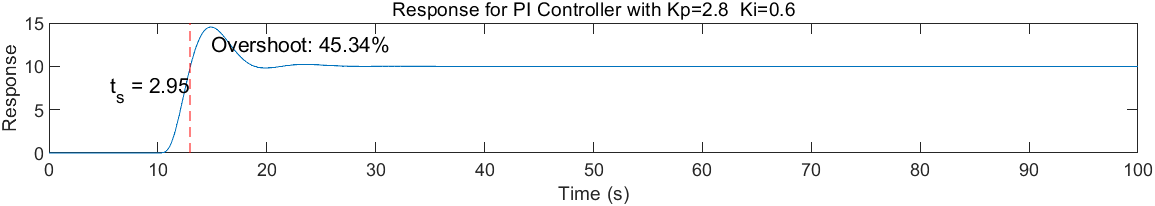
\includegraphics[width=1\linewidth]{./img/PI/p4.png}
  \end{figure}
  \begin{figure}[H]
    \centering
    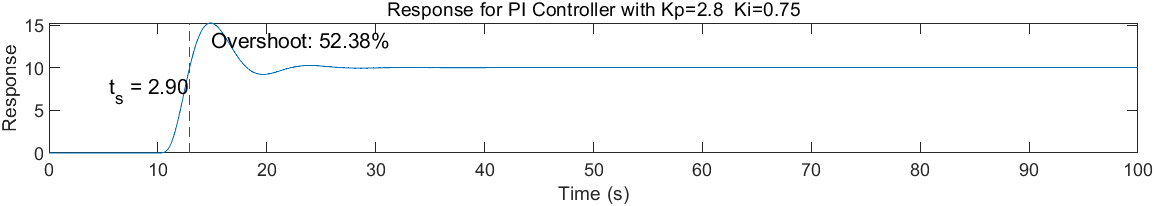
\includegraphics[width=1\linewidth]{./img/PI/p5.png}
  \end{figure}

\end{enumerate}

% =======================================================================================
\subsubsection{PD控制器}
参数:R = 10 (t>10);  N(s) = 0;  Td(s) = 0;

在这个模块中,将PD控制器接入了系统的Gc(s)的位置

实现了对两个参数 (Kp \& Kd) 进行了两组分析
\begin{enumerate}
  \item 保持Kp不变,调整Kd的值————以1为步长,在[1,5]的范围内生成5张系统时域图
  \begin{figure}[H]
    \centering
    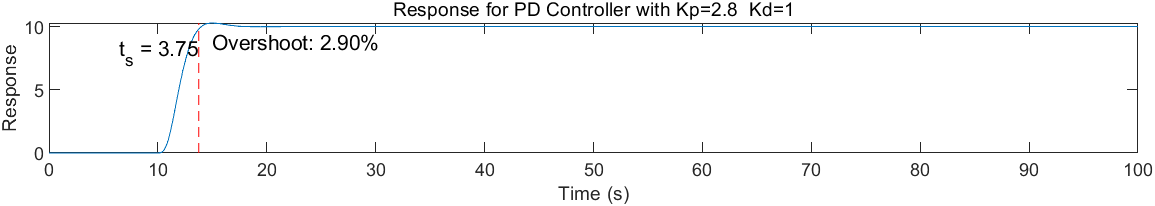
\includegraphics[width=1\linewidth]{./img/PD/p1.png}
  \end{figure}
  \begin{figure}[H]
    \centering
    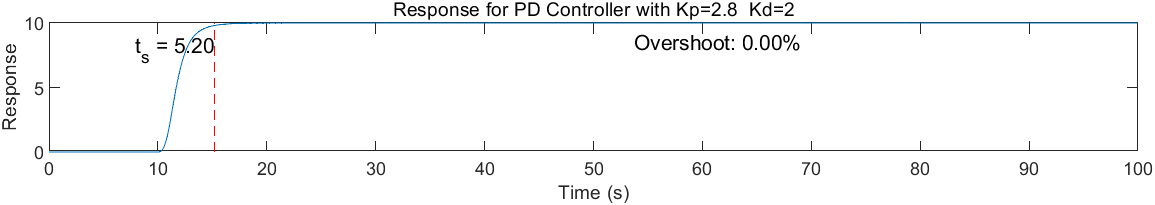
\includegraphics[width=1\linewidth]{./img/PD/p2.png}
  \end{figure}
  \begin{figure}[H]
    \centering
    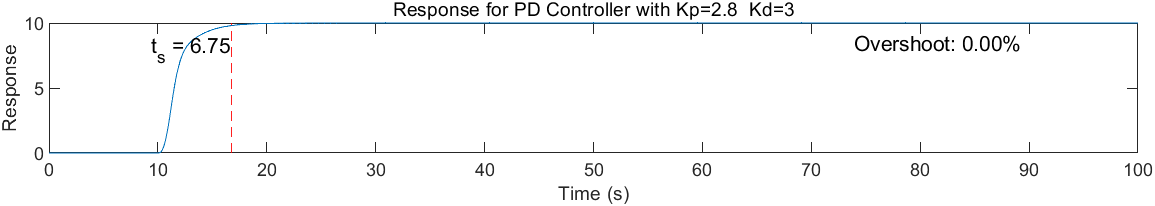
\includegraphics[width=1\linewidth]{./img/PD/p3.png}
  \end{figure}
  \begin{figure}[H]
    \centering
    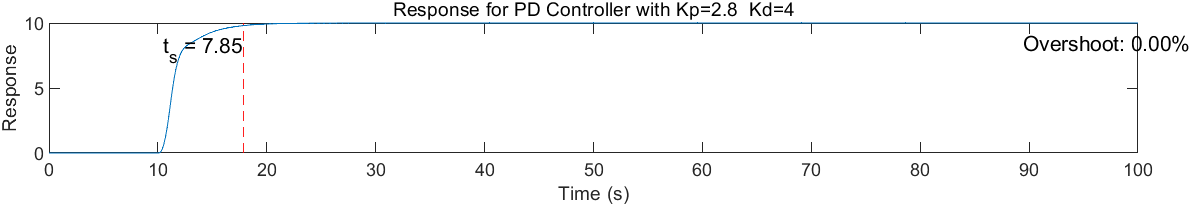
\includegraphics[width=1\linewidth]{./img/PD/p4.png}
  \end{figure}
  \begin{figure}[H]
    \centering
    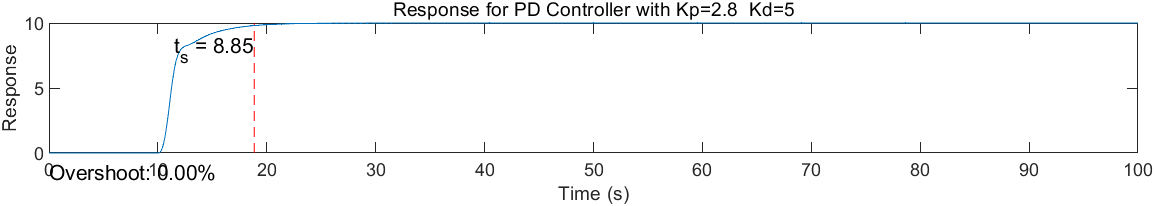
\includegraphics[width=1\linewidth]{./img/PD/p5.png}
  \end{figure}

  \item 保持Kd不变,调整Kp的值————以2为步长,在[2,10]的范围内生成5张系统时域图
  \begin{figure}[H]
    \centering
    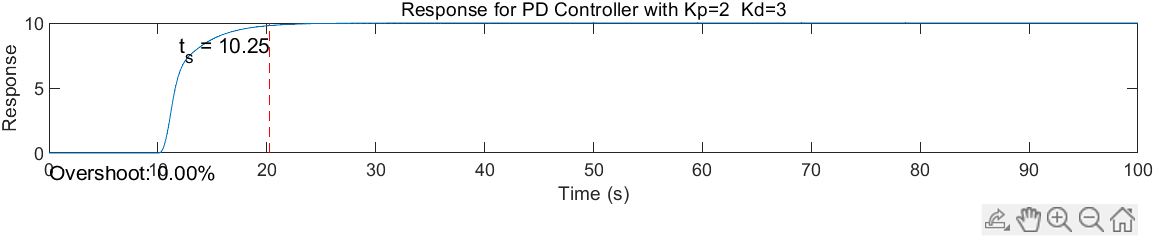
\includegraphics[width=1\linewidth]{./img/PD/d1.png}
  \end{figure}
  \begin{figure}[H]
    \centering
    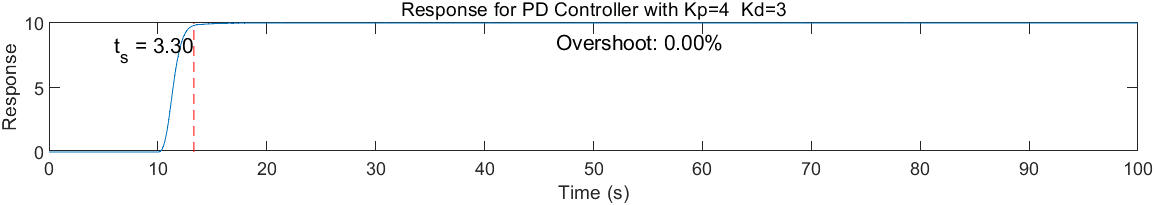
\includegraphics[width=1\linewidth]{./img/PD/d2.png}
  \end{figure}
  \begin{figure}[H]
    \centering
    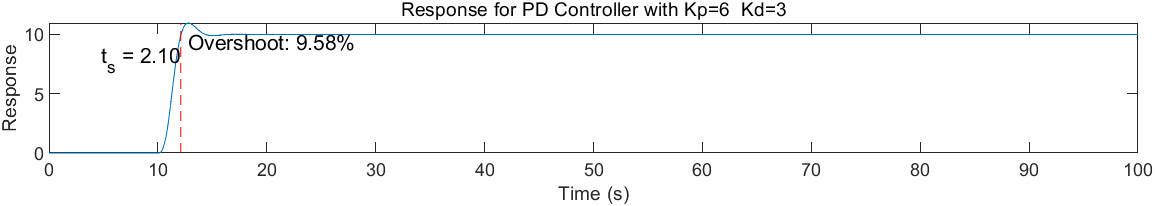
\includegraphics[width=1\linewidth]{./img/PD/d3.png}
  \end{figure}
  \begin{figure}[H]
    \centering
    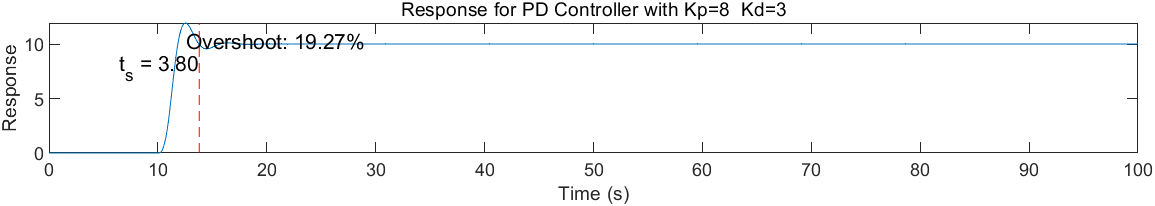
\includegraphics[width=1\linewidth]{./img/PD/d4.png}
  \end{figure}
  \begin{figure}[H]
    \centering
    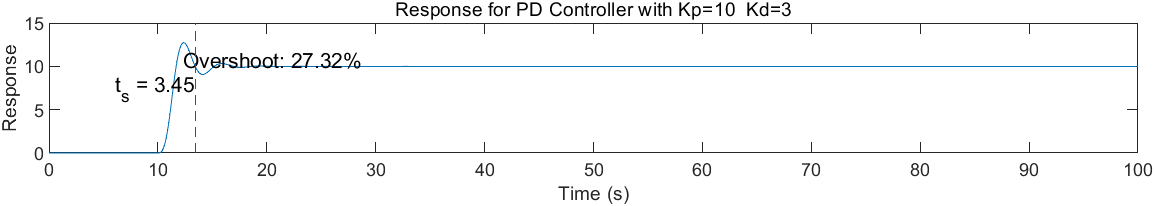
\includegraphics[width=1\linewidth]{./img/PD/d5.png}
  \end{figure}

\end{enumerate}

% =======================================================================================
\subsubsection{PID控制器}
参数:R = 10 (t>10);  N(s) = 0;  Td(s) = 0;

在这个模块中,将PiD控制器接入了系统的Gc(s)的位置

实现了对三个参数 (Kp \& Ki \& Kd) 进行了两组分析
\begin{enumerate}
  \item 保持Kp \& Ki不变,调整Kd的值————以0.8为步长,在[0.8,4]的范围内生成5张系统时域图
  \begin{figure}[H]
    \centering
    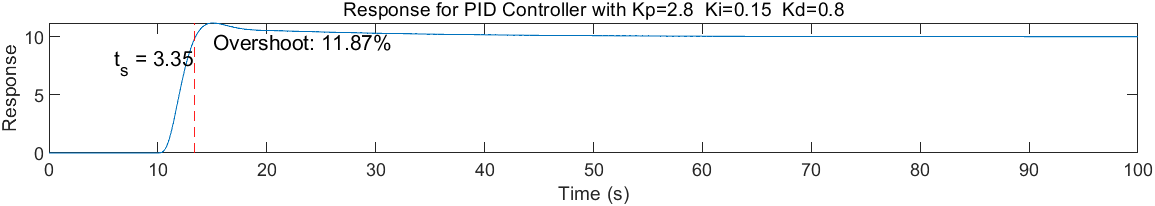
\includegraphics[width=1\linewidth]{./img/PID/pi1.png}
  \end{figure}
  \begin{figure}[H]
    \centering
    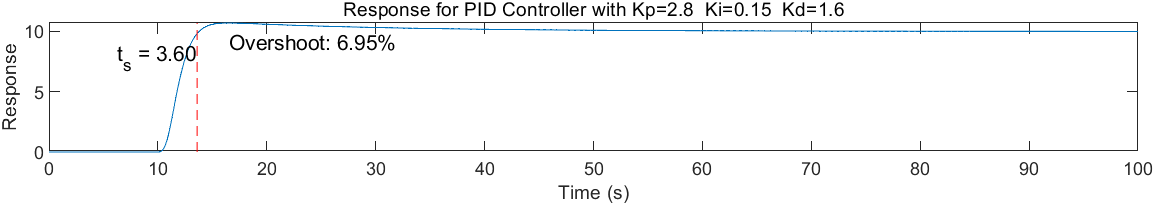
\includegraphics[width=1\linewidth]{./img/PID/pi2.png}
  \end{figure}
  \begin{figure}[H]
    \centering
    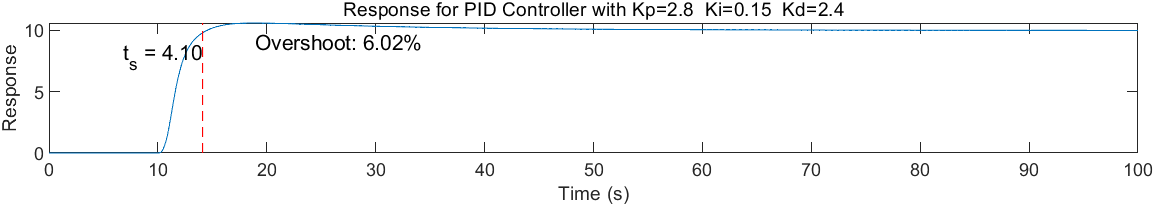
\includegraphics[width=1\linewidth]{./img/PID/pi3.png}
  \end{figure}
  \begin{figure}[H]
    \centering
    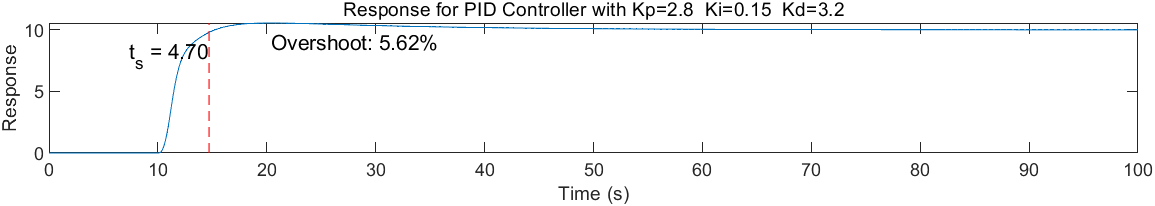
\includegraphics[width=1\linewidth]{./img/PID/pi4.png}
  \end{figure}
  \begin{figure}[H]
    \centering
    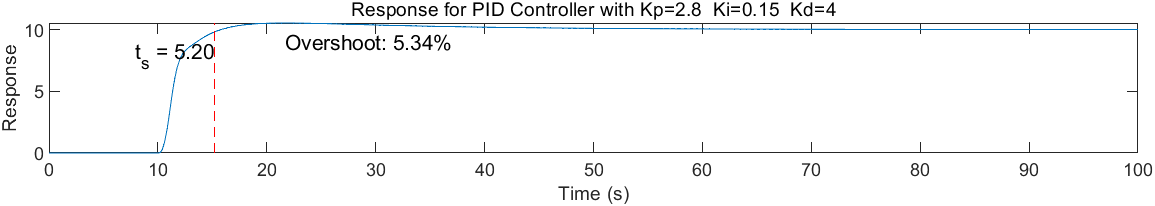
\includegraphics[width=1\linewidth]{./img/PID/pi5.png}
  \end{figure}

  \item 保持Kp \& Kd不变,调整Ki的值————以0.15为步长,在[0.15,0.75]的范围内生成5张系统时域图
  \begin{figure}[H]
    \centering
    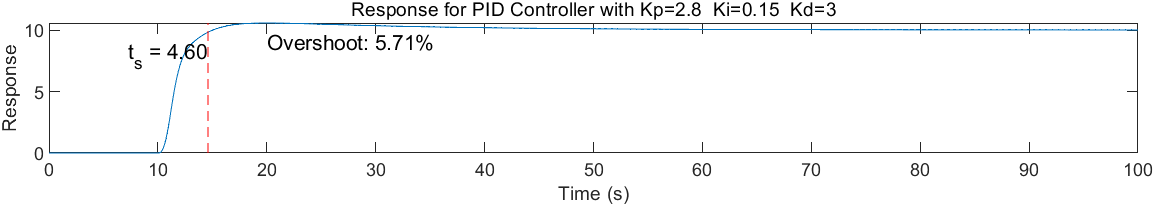
\includegraphics[width=1\linewidth]{./img/PID/pd1.png}
  \end{figure}
  \begin{figure}[H]
    \centering
    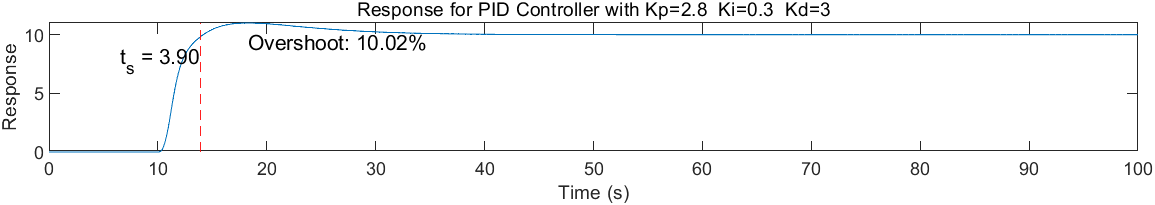
\includegraphics[width=1\linewidth]{./img/PID/pd2.png}
  \end{figure}
  \begin{figure}[H]
    \centering
    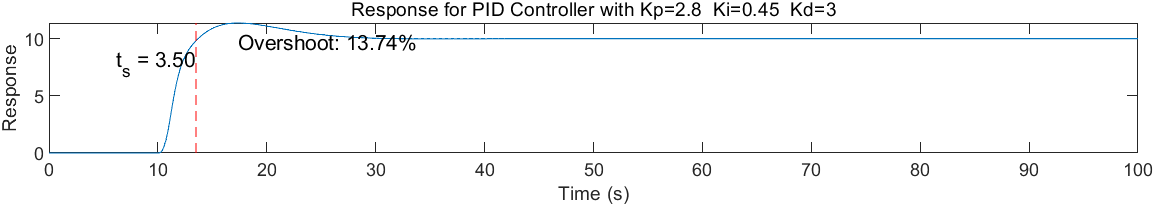
\includegraphics[width=1\linewidth]{./img/PID/pd3.png}
  \end{figure}
  \begin{figure}[H]
    \centering
    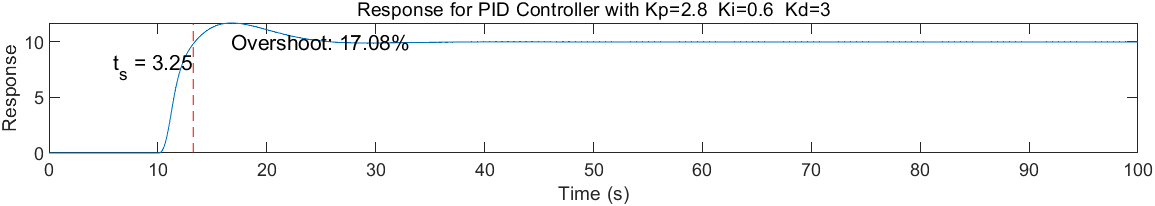
\includegraphics[width=1\linewidth]{./img/PID/pd4.png}
  \end{figure}
  \begin{figure}[H]
    \centering
    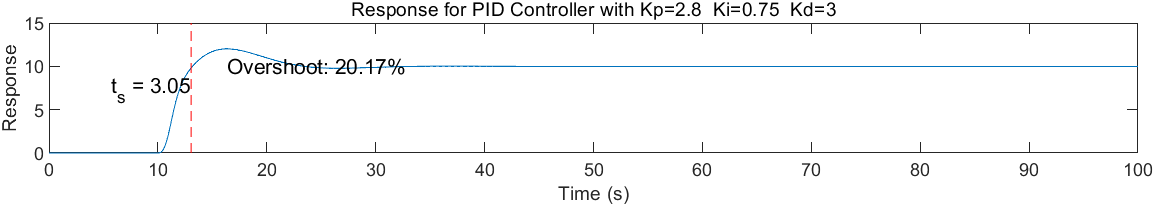
\includegraphics[width=1\linewidth]{./img/PID/pd5.png}
  \end{figure}

\item 保持Ki \& Kd不变,调整Kp的值————以0.6为步长,在[0.6,3]的范围内生成5张系统时域图
  \begin{figure}[H]
    \centering
    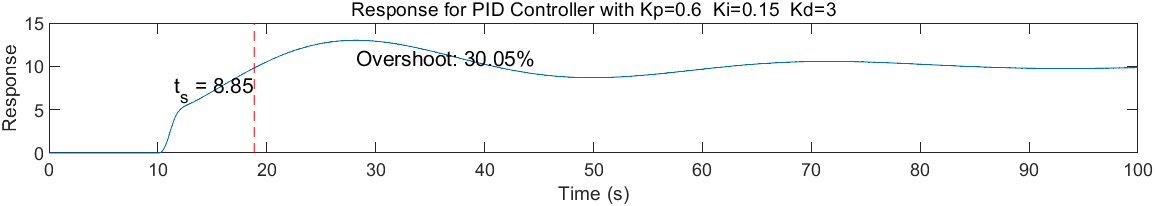
\includegraphics[width=1\linewidth]{./img/PID/id1.png}
  \end{figure}
  \begin{figure}[H]
    \centering
    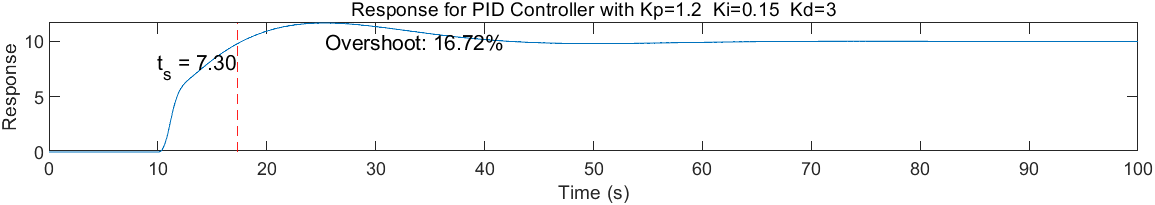
\includegraphics[width=1\linewidth]{./img/PID/id2.png}
  \end{figure}
  \begin{figure}[H]
    \centering
    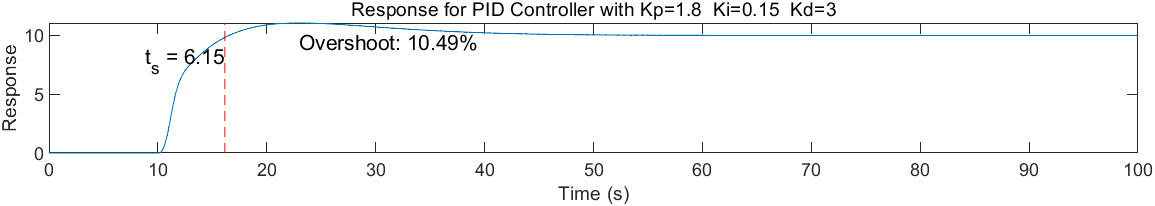
\includegraphics[width=1\linewidth]{./img/PID/id3.png}
  \end{figure}
  \begin{figure}[H]
    \centering
    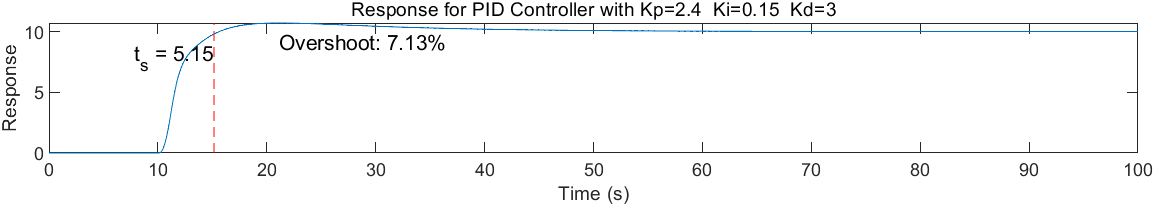
\includegraphics[width=1\linewidth]{./img/PID/id4.png}
  \end{figure}
  \begin{figure}[H]
    \centering
    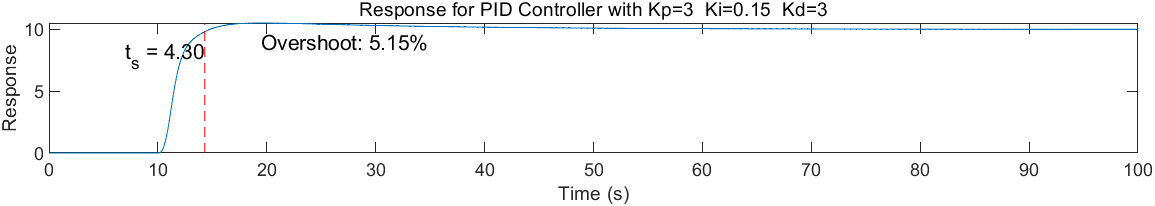
\includegraphics[width=1\linewidth]{./img/PID/id5.png}
  \end{figure}

\end{enumerate}

% ====================================================
\subsubsection{阶跃扰动响应下的PID控制器}
参数:R = 10 (t>10);  N(s) = 0;  Td(s) = 50/s (t>50);

在这个模块中,将PID控制器接入了系统的Gc(s)的位置

在t = 0的时候系统对R阶跃信号产生响应,当趋于稳定以后,对系统添加一个Td(s) = 50/s的阶跃扰动响应信号
观察系统的变化,同时与没有接入PID控制器的信号进行对比

实现了对三个参数 (Kp \& Ki \& Kd) 进行了两组分析
\begin{enumerate}
  \item 保持Kp \& Ki不变,调整Kd的值————以0.8为步长,在[0.8,4]的范围内生成5张系统时域图
  \begin{figure}[H]
    \centering
    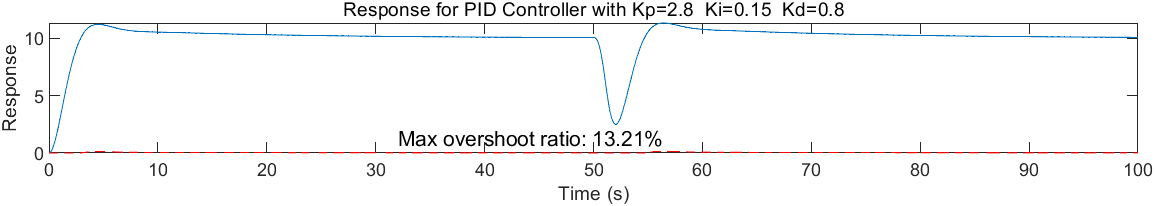
\includegraphics[width=1\linewidth]{./img/PID_with_noise/pi1.png}
  \end{figure}
  \begin{figure}[H]
    \centering
    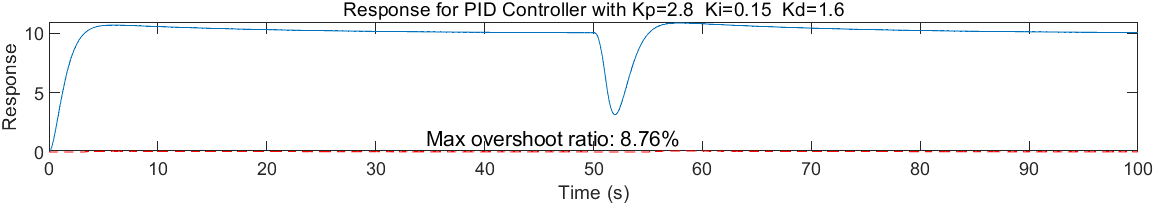
\includegraphics[width=1\linewidth]{./img/PID_with_noise/pi2.png}
  \end{figure}
  \begin{figure}[H]
    \centering
    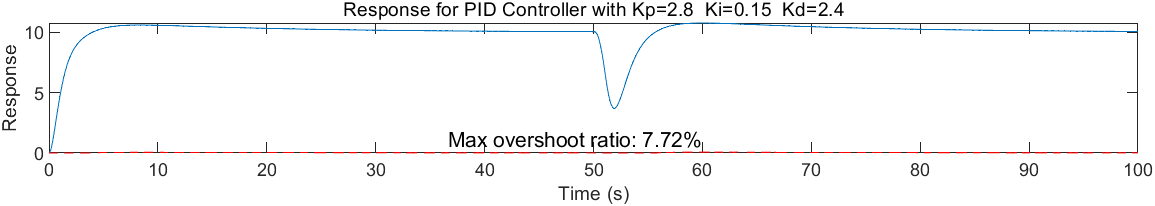
\includegraphics[width=1\linewidth]{./img/PID_with_noise/pi3.png}
  \end{figure}
  \begin{figure}[H]
    \centering
    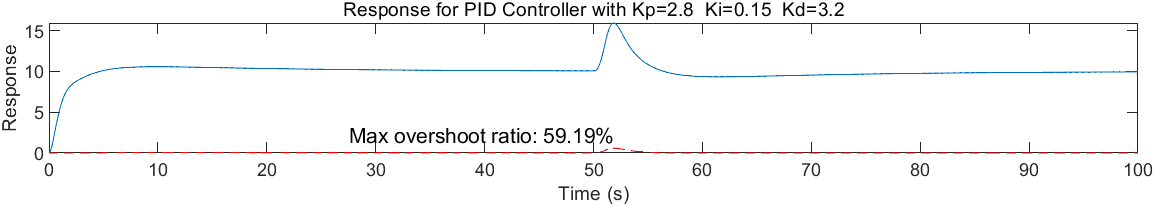
\includegraphics[width=1\linewidth]{./img/PID_with_noise/pi4.png}
  \end{figure}
  \begin{figure}[H]
    \centering
    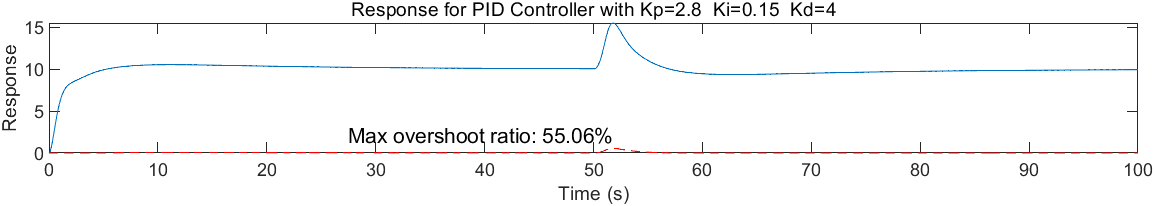
\includegraphics[width=1\linewidth]{./img/PID_with_noise/pi5.png}
  \end{figure}

  \item 保持Kp \& Kd不变,调整Ki的值————以0.15为步长,在[0.15,0.75]的范围内生成5张系统时域图
  \begin{figure}[H]
    \centering
    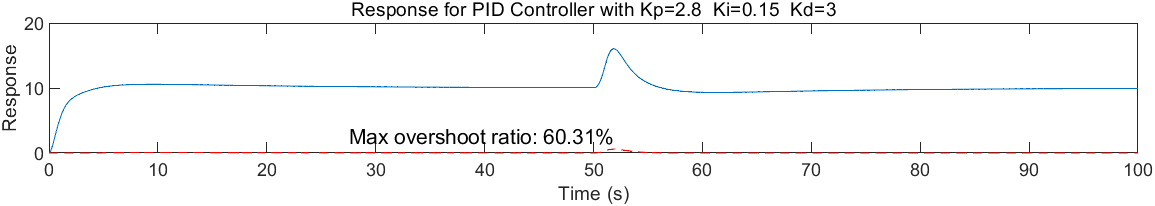
\includegraphics[width=1\linewidth]{./img/PID_with_noise/pd1.png}
  \end{figure}
  \begin{figure}[H]
    \centering
    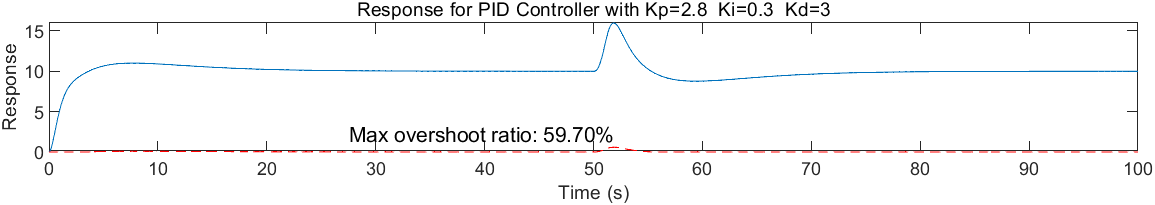
\includegraphics[width=1\linewidth]{./img/PID_with_noise/pd2.png}
  \end{figure}
  \begin{figure}[H]
    \centering
    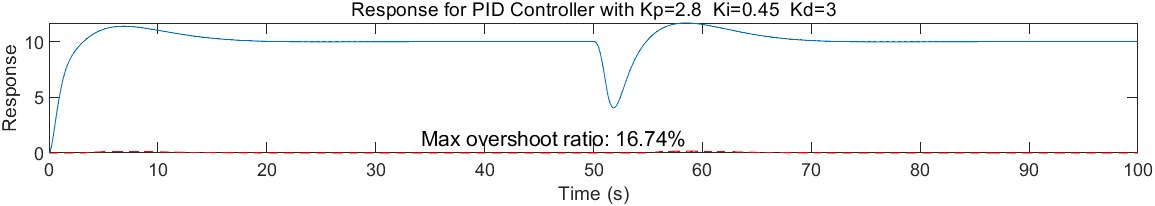
\includegraphics[width=1\linewidth]{./img/PID_with_noise/pd3.png}
  \end{figure}
  \begin{figure}[H]
    \centering
    \includegraphics[width=1\linewidth]{./img/PID_with_noise/pd4.png}
  \end{figure}
  \begin{figure}[H]
    \centering
    \includegraphics[width=1\linewidth]{./img/PID_with_noise/pd5.png}
  \end{figure}

\item 保持Ki \& Kd不变,调整Kp的值————以0.6为步长,在[0.6,3]的范围内生成5张系统时域图
  \begin{figure}[H]
    \centering
    \includegraphics[width=1\linewidth]{./img/PID_with_noise/id1.png}
  \end{figure}
  \begin{figure}[H]
    \centering
    \includegraphics[width=1\linewidth]{./img/PID_with_noise/id2.png}
  \end{figure}
  \begin{figure}[H]
    \centering
    \includegraphics[width=1\linewidth]{./img/PID_with_noise/id3.png}
  \end{figure}
  \begin{figure}[H]
    \centering
    \includegraphics[width=1\linewidth]{./img/PID_with_noise/id4.png}
  \end{figure}
  \begin{figure}[H]
    \centering
    \includegraphics[width=1\linewidth]{./img/PID_with_noise/id5.png}
  \end{figure}

\end{enumerate}

没有PID控制器的原系统响应为
\begin{figure}[H]
\centering
\includegraphics[width=0.8\linewidth]{./img/None_p2_Td.png}
\end{figure}
可以看到,当加入了PID系统以后,整体的超调量有了明显的下降,
这体现了通过加入PID控制器以后,系统的稳定性大大提高了。
这对于手术过程中的病人麻醉状态的稳定有着至关重要的作用。


\section{实验分析与结论}
\subsection{结论}
利用控制变量法及相关资料,我在
PI/PD/PID 三种控制器的有无扰动两种情况下最
终人工调整三个参数获得以下结论:

\begin{table}[!ht]
  \centering
  \captionnamefont{\wuhao\bf\heiti}
  \captiontitlefont{\wuhao\bf\heiti}
  \caption{PID参数对系统的影响} 
  \begin{tabular}{llllll}
      \toprule
      调整方式 & 上升时间 & 超调量 & 稳态误差 & 稳定性 \\ 
      \midrule
      ↑ Kp & ↓ 减少 & ↑ 增加 & ↓ 减少 & ↓ 变差 \\ 
      ↑ Ki & ↓ 小幅减少 & ↑ 增加 & ↓ 大幅减少 & ↓ 变差 \\ 
      ↑ Kd & ↓ 小幅减少 & ↓ 减少 & → 变动不大 & ↑ 变好 \\
      \bottomrule
  \end{tabular}
\end{table}

\subsection{最优参数}
人工调整有一种作法是先将 Ki 及 Kd 设为零,
增加 Kp 一直到回路输出震荡为止,之后再将 Kp
设定为“1/4 振幅衰减” (使系统第二次过冲量是第
一次的 1/4 ) 增益的一半,然后增加 Ki 直到一定
时间后的稳态误差可被修正为止。不过若 Ki 可能
会造成不稳定,最后若有需要,可以增加 Kd ,并
确认在负载变动后回路可以够快的回到其设定值,
不过若 Kd 太会造成响应太快及过冲。一般而言快
速反应的 PID 应该会有轻微的过冲,只是有些系
统不允许过冲。因此需要将回授系统调整为过阻
尼系统,而 Kp 比造成震荡 Kp 的一半还要小很多。\cite{PID}

当然历史上 PID 的参数调试还有很多,例如
齐格勒-尼克尔斯方法等,大部分现代的工业设备
也实现了 PID 自动调试及最佳化软件。

\section*{写在最后}
在完成自动控制原理课程作业的这个过程中,我体验到了丰富而深刻的学习过程,
由衷地感谢所有帮助我、支持我的人。

首先,我要感谢李中华老师,您的热情教课和专业引导使我对PID控制和信号流图有了深入的理解和掌握。
每次课堂上的讲解都是精心准备的,它们如照亮黑夜的明灯,
指引我探索控制理论的广阔领域。您给予我们的这次作业机会,
是我进一步理解自动控制原理的一个宝贵的实践场所。我深深地感谢您的悉心教诲,
也感谢您给我提供了这样一个展现所学知识的机会。

我也要特别感谢方桂安学长。虽然去年的作业要求与今年的不同,
但学长去年在博客上分享的报告对我产生了深远的影响。在您的报告中,
我看到了深入浅出的解析和清晰的逻辑思维。您的报告让我深受启发,
也使我对PID控制和信号流图的学习有了更深的认识和理解。我把您的博客网址和引用都标在了文末,
以表达我对您贡献的尊重和感谢。

回顾完成这份作业的整个过程,我深感欣喜。通过这次实践,我得以将所学的理论知识与实际操作相结合,
实现了知识与实践的完美结合。我深深感受到自动控制原理的独特魅力和应用价值。

本着开源精神,我也将本次作业的MATLAB代码和完成报告所用的\LaTeX 源文件全部托管在了GitHub仓库中,
以便老师和同学们进行浏览和学习。这不仅是我对自己工作的一种展示,
也是希望能通过大家的交流和互动,一起探索学习,一起进步。

我诚挚地邀请每一位对此感兴趣的老师和同学,前往我的GitHub仓库查阅代码,
提出您的宝贵建议和批评。任何形式的反馈和建议,无论是关于代码的优化,
还是对于实验方法和结果的讨论,我都将热烈欢迎。通过大家的共同努力,
我们可以一起推进学术的发展,也可以一起提升我们自己。

GitHub repository URL: 

\href{https://github.com/pbcn2/PID-control-in-blood-pressure-control-in-anesthesia-process}{https://github.com/pbcn2/PID-control-in-blood-pressure-control-in-anesthesia-process}

%%%%%%%%%%%%%%%%%%%%%%%%%%%%%%%%%%%%%%%%%%%%%%%%%%%%%%%%%%%%%%%%
%  参考文献
%%%%%%%%%%%%%%%%%%%%%%%%%%%%%%%%%%%%%%%%%%%%%%%%%%%%%%%%%%%%%%%%
%  参考文献按GB/T 7714-2015《文后参考文献著录规则》的要求著录. 
%  参考文献在正文中的引用方法:\cite{bib文件条目的第一行}

\renewcommand\refname{\heiti\wuhao\centerline{参考文献}\global\def\refname{参考文献}}
\vskip 12pt

\let\OLDthebibliography\thebibliography
\renewcommand\thebibliography[1]{
  \OLDthebibliography{#1}
  \setlength{\parskip}{0pt}
  \setlength{\itemsep}{0pt plus 0.3ex}
}

{
\renewcommand{\baselinestretch}{0.9}
\liuhao
\bibliographystyle{gbt7714-numerical}
\bibliography{./TempExample}
}



\end{document}

